\documentclass[PMI,VKR]{HSEUniversity}
% Возможные опции: KR или VKR; PI или BI

\title{Dynamic Topic Modeling for Voice Dialogues}
\author{Miakov Timofey Ilich}
\supervisor{Professor NRU HSE - Nizhniy Novgorodw}{L.V. Savchenko }
\Year{2024}
\Abstract{

}

\bibliography{library.bib}

\begin{document}
\maketitle

\chapter{Introduction}

\section{Motivation}

\section{Research Objectives}


\chapter{Theoretical explanation}

The pipeline of dynamic thematic modelling of audio dialogues, which will be considered in this paper, is divided into several main stages. 
These include segmentation, topic extraction, and topic evolution. 
The approaches and algorithms used in these stages will be described in detail from a theoretical point of view.

\section{Dialogue Segmentation Stage}

Для решения задач в сфере обработки естественного языка до определенного момента широко применялись рекурентный нейронные сети (RNN). Основной архитектурой в таких задачах была модель encoder-decoder\cite{seq2seq:2014} (рис A), в которой каждый из блоков  представлял из себя RNN.
На вход энкодеру подавались последовательно токены, после чего на выход получался ембеддинг, который в свою очоередь подавался декодеру. Декодер, используя токены изначального предложения, а также переданное представление от кодировщика, генерирует целевую последовательность.

\begin{figure}[h]
    \centering
    \includegraphics[scale=0.21]{img/transformer/enc_dec.png}
    \caption{Архитекутура encoder-decoder}
\end{figure}

Но у такой архитекутры были некоторые проблемы. Во-первых, все предствлание текста сжималось в один вектор, чаще всего это из-за многообразие возможных входных данных и огранниченности вектора терялась важная информация. Во-вторых, декодеру могла понадобиться разная информация от энкодера на разных этапах генерации, но декодер видит только одно представление источника.

Чтобы исправить эти проблемы, представили механизм внимания (attention mechanism\cite{attention:2014}).

\section{Text embeddings extraction}

Механизм внимания является частью нейронной сети. На каждом этапе декодирования он решает, какие части входных данных важнее всего. При этом кодировщику не нужно сжимать весь исходный код в один вектор - он создает представления для всех токенов источника.

\begin{figure}[h]
    \centering
    \includegraphics[scale=0.3]{img/transformer/attention_mech1.png}
    \caption{Схема работы механизма внимания}
\end{figure}

\newpage
Алгоритм работы механизма внимания в encoder-decoder модели приведен ниже.

\begin{itemize}
    \item На каждом этапе декодирования механизм внимания получает на вход: состояние декодера $h_t$ и все состояния кодировщика $s_1, s_2, \dots, s_m$
    \item Вычисляет коэффициенты внимания (attention scores) для каждого состояния кодеровщика $s_k$ механизм внимания вычисляет свою "релевантность" для этого состояния декодера $h_t$. \\
          Для вычисления можно применить любую функцию, однако, есть несколько популярных и простых вариантов, которые работают довольно хорошо.
          \begin{itemize}
              \item $scores(h_t, s_k) = h_t^T \cdot s_k $
              \item $scores(h_t, s_k) = h_t^T \cdot W \cdot s_k $, где $W$ - матрица (обучаемый параметр)
              \item $scores(h_t, s_k) = w_2^T \cdot \tanh(W \cdot [h_t^T, s_k]) $, где $W, w_2$ - матрицы (обучаемые параметры), а $[h_t^T, s_k]$ означает конкатенацию векторов
          \end{itemize}

    \item Вычисляет веса внимания (attention weights): распределение вероятностей - softmax, применяемое к показателям внимания;
    \item Вычисляет вывод внимания : взвешенная сумма состояний декодера с весами внимания.
\end{itemize}

\begin{figure}[h]
    \centering
    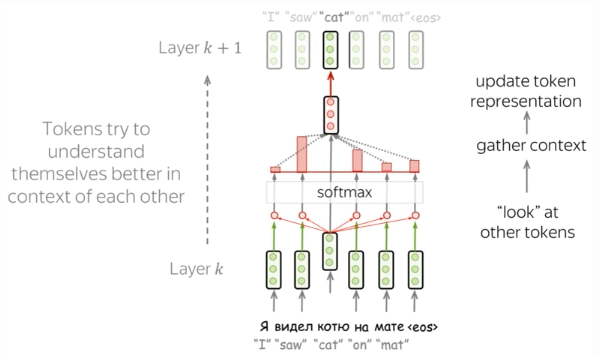
\includegraphics[scale=1]{img/transformer/self-attention.png}
    \caption{Схема работы self-attention механизма}
\end{figure}

\subsection{Architecture of BERT model}

Self-attention - является одним из ключевых компонентов модели, в которой токены взаимодействуют друг с другом. На каждом шаге в энкодере токены обмениваются информацией между собой, собирает контекст и обновляет предыдущее представление себя (рис 2.3). Такой подход полностью исключает последовательную обработку, как в RNN, что ускоряет работу нейронной сети и дает возможность обрабатывать каждое слово параллельно.

\newpage
\subsection{}

Каждый входной токен в self-attention получает три представления, соответствующие ролям, которые он может играть:
\begin{itemize}
    \item query - запрашивает информацию;
    \item key - показывает, какая информация есть у него;
    \item value - дает запрашиваемую информацию;
\end{itemize}

От слова, которое мы сейчас подаем на вход (центральное), требуется query вектор, этим вектором мы запрашиваем у других информацию о текущем слове в данном контексте. От каждого другого слова нам будет нужен вектор key, который показывает, какую информацию данное слово может сказать о смысле центрального слова, а также вектор value, из которого мы и получим нужную нам информацию.

Получив информацию от каждого вектора, мы подаем это на вход softmax функции и получаем итоговый эмбеддинг центрального слова.
На рисунке нижен представлен полный алгоритм взаимодействия Q, K, V в self-attention механизме.

\newpage
\begin{figure}[h]
    \centering
    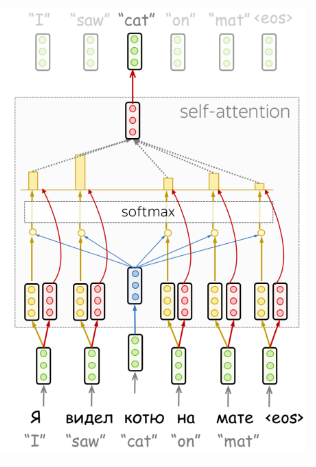
\includegraphics[scale=1]{img/transformer/query-key-value.png}
    \caption{Query, Key, Value в self-attention механизма}
\end{figure}

Формула для вычисления выходных данных внимания следующая:

\begin{center}
    $Attention(q, k, v) = softmax(\frac{q \cdot k^T}{\sqrt{d_k}}) \cdot v $
\end{center}

\subsection{Masked self-attention}

Для энкодера и декодера используются разные способы получения токенов, если энкодер получает все токены сразу и каждый токен может смотреть на любой другой токен во входном предложении, в декодере, мы генерируем по одному токену за раз: во время генерации мы не знаем, какие токены мы будем генерировать в дальше.
Чтобы запретить декодеру заглядывать вперед, модель использует masked-self attention, который видит токены, только стоящие до него во входной последовательности.

Работа masked self-attention отличается во время обучения и инференса модели. Во время второго декодер не заглядывает вперед - так как, мы не знаем, что будет дальше. Но при обучении используются уже известные нам данные. Поэтому при обучении на вход декодеру подется все целевое предложение целиком - без масок.

На рисунке нижне приведен алгоритм работы masked self-attention механизма.

\begin{figure}[h]
    \centering
    \includegraphics[scale=0.9]{img/transformer/masked self-attention.png}
    \caption{Схема работы masked Self-attention механизма}
\end{figure}

\begin{figure}[h]
    \centering
    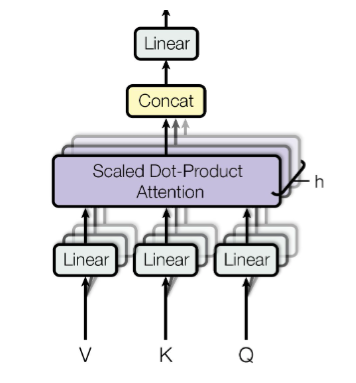
\includegraphics[scale=1]{img/transformer/multi-head.png}
    \caption{Схема Multi-head attention}
\end{figure}

\subsection{Multi-Head Attention}

Обычно понимание роли слова в предложении требует понимания того, как оно связано с разными частями предложения. Это важно не только при обработке исходного предложения, но и при генерации целевого.
Поэтому мы должны позволить модели сосредоточиться на разных вещах: для этого сделали multi-head attention. Вместо одного attention механизма multi-head attention имеет несколько «голов», которые работают независимо.

\begin{center}
    $MultiHead(Q, K, V) = Concat(head_{1}, head_{2}, \dots, head_{n})$ \\
    $head_{i} = Attention(QW^{i}_{Q}, KW^{i}_{K}, VW^{i}_{V})$
\end{center}

Формально это реализовано в виде нескольких механизмов внимания, результаты которых объединяются. (рис 2.6)

\newpage
\section{Трансформер: Архитектура модель}

Трансформер - это модель, основанная только на механизме винмания и оказавшая огромное влияние на NLP в частности и машинном обучении в целом. Впервые представленная в статье Attention is All You Need\cite{allyouneed:2017} в 2017 году.
Модель сразу показала лучшие результаты в задаче перевода, в сравнении с encoder-decoder модели.

\begin{figure}[h]
    \centering
    \includegraphics[scale=0.2]{img/transformer/transformer.png}
    \caption{Схема архитектуры Траснформер}
\end{figure}

Трансформер состоит из частей, которое ранне описывались. Encoder состоит из multi-head self-attention механизмов и генерирует представление слов, а decoder из masked self-attention механизма, который уже генерирует новую последовательность. Это происходит в несколько слоев, обычно 6.

Теперь рассмотрими другие составляющие архитекутры:\\


\subsection{Feed forward and Add $\&$ Norm}

Кроме блоков внимания, в Трансформере также присутствуют feed forward слои, которые состоят из линейного слоя и фукнции активации ReLU.

\begin{figure}[h]
    \centering
    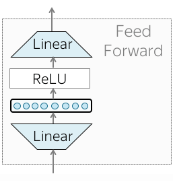
\includegraphics[scale=1]{img/transformer/feed_forward.png}
    \caption{Feed-forward слой}
\end{figure}

Вторым важным слоем является LayerNorm, которой независимо нормализует векторное представление каждой последовательности в батче. В Трансформере нормализуются векторное представление каждого токена. Кроме того, LayerNorm имеет обучаемые параметры, $scale$ и $bias$, которые используются после нормализации для масштабирования выходных данных слоя.

\begin{figure}[h]
    \centering
    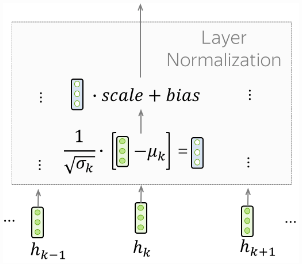
\includegraphics[scale=1]{img/transformer/layer_norm.png}
    \caption{LayerNorm слой}
\end{figure}

На рис 2.8 стоит обратить внимание на то, что $\mu_{k}$ и $\sigma_{k}$ оцениваются для каждой последовательности, в отличии от $scale$ и $bias$, которые являются параметрами слоя.


\subsection{Positional encoding}

Поскольку Transformer не знает порядок входных токенов, т.к все токены обрабатываются одновременно, поэтому мы должны явно показать модели положения токенов. Для этого у нас есть два набора вложений: для самихтокенов и для их позиций. Тогда входное представление токена является сумма двух вложений.
Positional encodings можно обучить, но авторы оригинальной статьи обнаружили, что наличие исправленных вложений не ухудшает качество модели. Итоговая формула для позиционные вложения выглядят так:
\begin{center}
    $PE_{pos,2i} = \sin(pos/10000^{2i/d_{model}})$, \\
    $PE_{pos,2i+1} = \cos(pos/10000^{2i/d_{model}})$, \\
\end{center}

где $pos$ это позиция и $i$ является векторным измерением. Каждое измерение позиционного кодирования соответствует синусоиде, а длины волн образуют геометрическую прогрессию от $2\pi$ до 10000 $\cdot 2\pi$.

\begin{figure}[h]
    \centering
    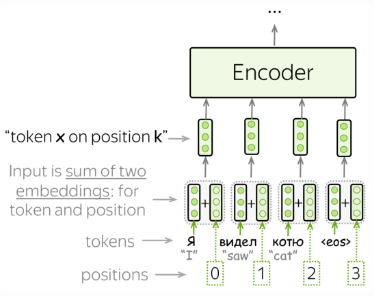
\includegraphics[scale=1]{img/transformer/pos_encoding.png}
    \caption{Positional encoding}
\end{figure}


\subsection{Residual connection}

Как и в сверточных сетях, в Трансформере применяется residual connections. Смысл residual connection очень прост, добавляет входные данные к выходным данным модели, но в то же время это очень полезная вещь: он борется с проблемой затухания градиента по сети и позволяют использовать много слоев.

\begin{figure}[h]
    \centering
    \includegraphics[scale=0.9]{img/transformer/res_block.png}
    \caption{Residual connection}
\end{figure}

В трансформаторе остаточные соединения используются после каждого блока внимания и полносвязного блока.

\section{Модель TimeSformer}
\subsection{Новый подход к решению задач компьютерного зрения}

Сверточные нейронные сети (CNN) являлись базовой архитектурой для задач распознавания изображений и показывали лучшие результаты во всех бенчмарках. Базовым слоем таких сетей являлись свертки, которые обрабатывали все изображения сразу.

Однако в 2016 году Google опубликовали статью, в которой представили новую нейронную сеть для работы с изображениями - Vision Transformer\cite{vit:2016} (далее ViT). Основным отличием от других нейронных сетей для обработки изображений стало использование архитекутры Transformer вместо сверток.

Ключевая идея, лежащая в основе ViT, заключается в обработке изображения как набор патчей (patches), а затем использовании модели на основе Transformer для обработки этих патчей. Участки сначала сглаживаются в набор векторов, которые затем обрабатываются. Это позволяет модели находить и запоминать долгосрочные зависимости между различными патчами, что потенциально приводит к повышению качества модели по сравнению с традиционными CNN.

Так как основной темой работы, являются видео, основной моделью стал не ViT, а еще более новая модель, разработанная Facebook, которая называется TimeSFormer.
TimeSformer\cite{timesformer:2021} адаптирует стандартную архитектуру Трансформер и приемы, используемые в ViT, к видео, позволяя изучать пространственно-временные характеристики непосредственно из последовательности исправлений на уровне кадров.

\subsection{Обработка входного изображения}

На вход в модель подается разбитое на N частей изображение. Т.к. Трансформер принимает на вход 1D-вектора,  части изображения с помощью линейно проекции \textquotedblrightвытягивают\textquotedblright из 2D в 1D.
Также как и в задачах обработки текста, на вход в модель кроме патчей надо подать positional encoders.
Итоговые преобразования изображения выглядят так: \\

\noindent$z_{0} = [x_{class}; x^1_{p} \cdot E; x^2_{p} \cdot E; \dots x^N_{p} \cdot E] + E_{pos} $,\\
$x \in \mathds{R}^{H \times W \times C}$, $E \in \mathds{R}^{N \times (P^{2} \times C)}$,
где $C$ - кол-во каналов, $(P, P)$ - размер каждого патча, $N = HW / P^2$

\begin{figure}[h]
    \centering
    \includegraphics[scale=1]{img/vit/patches.png}
    \caption{Подготовка патчей}
\end{figure}

В качестве альтернативы патчам изображения, входная последовательность может быть сформирована
из карт характеристик (feature map) CNN. В этой гибридной модели проекция E применяется к участкам, извлеченным из карты объектов CNN, как частный случай, патчи могут иметь пространственный размер 1x1.
Патч с классом изображения и positional embeddings добавляются, как описано выше.


\subsection{Query-Key-Value вычисления}

TimeSFormer состоит из L блоков энкодера. В каждом блоке $l$, как и в оригинальном трансформере вычисляются Query, Key, Value для каждого патча из его прошлого состояния $z_{(p, t)}^{(l-1)}$

\begin{center}
    $q_{(p, t)}^{(l, a)} = W_{Q}^{(l, a)} \cdot LN(z_{(p, t)}^{(l-1)}) \in \mathds{R}^{D_{h}}$,

    $q_{(p, t)}^{(l, a)} = W_{K}^{(l, a)} \cdot LN(z_{(p, t)}^{(l-1)}) \in \mathds{R}^{D_{h}}$,

    $q_{(p, t)}^{(l, a)} = W_{V}^{(l, a)} \cdot LN(z_{(p, t)}^{(l-1)}) \in \mathds{R}^{D_{h}}$,
\end{center}
где $LN()$ означате LayerNorm, $a = 1, \dots, A$ - индексы голов в Multi-head attention.

\subsection{Attention weights}
Вычисление self-attention коэффициентов для $a_{(p, t)}^{(l, a)}$ для патча $(p, t)$ вычисляется как:

\begin{center}
    $a_{(p, t)}^{(l, a)} = SoftMax(\frac{q_{(p, t)}^{(l, a)}}{\sqrt{D_{h}}}^{T} \cdot \left[k_{(0, 0)}^{(l, a)} {k_{(p', t')}^{(l, a)}}_{p' = 1, \dots, N, t' = 1, \dots, F} \right])$
\end{center}

\subsection{Encoding}

Закодированное представление $z_{(p, t)}^{(l)}$ в блоке $l$ получается путем вычисления взвешенной суммы векторов значений с использованием коэффициентов self-attention от каждой головы multi-head attention:

\begin{center}
    $s_{(p, t),(0, 0)}^{(l, a)} = a_{(p, t),(0, 0)}^{(l, a)} \cdot v_{(0, 0)} + \sum\limits_{p'=1}^N \sum\limits_{t'=1}^F a_{(p, t),(p', t')}^{(l, a)} \cdot a_{(p', t')}^{(l, a)}$
\end{center}

Затем векторы каждого головы конкатенируются, проецируется и передается через MLP, используя residual connections после каждой операции:

\begin{center}
    $z'_{(p, t)}^{(l)} = W_{O} \cdot \begin{bmatrix}
            s_{(p, t)}^{(l, 1)} \\
            \vdots              \\
            s_{(p, t)}^{(l, A)}
        \end{bmatrix} + z_{(p, t)}^{(l - 1)}$

    $z_{(p, t)}^{(l)} = MLP(LN(z'_{(p, t)}^{(l)})) + z'_{(p, t)}^{(l)}$
\end{center}

Для финальной классификации используется MLP с 1 скрытым слоем. \\

Ниже представлен блок энкодера в TimeSFormer:

\begin{figure}[h]
    \centering
    \includegraphics[scale=.9]{img/vit/timesformer.png}
    \caption{Энкодер блок в TimeSFormer}
\end{figure}

\newpage
\section{Модель RoBERTa}

\subsection{BERT}

BERT был представлен в статье BERT: Pre-training of Deep Bidirectional Transformers for Language Understanding\cite{bert:2018}. Архитектура модели BERT - это энкодер Transformer. По новому подошли к процессу обучения и к тому, как BERT используется для последующих задач.

\begin{figure}[h]
    \centering
    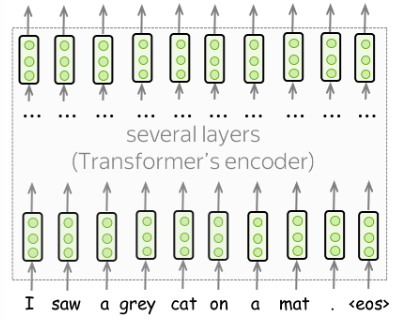
\includegraphics[scale=0.8]{img/bert/bert.png}
    \caption{Архитектура BERT}
\end{figure}

\begin{center}
    \textbf{Новый способ обучения}
\end{center}

\begin{figure}[h]
    \centering
    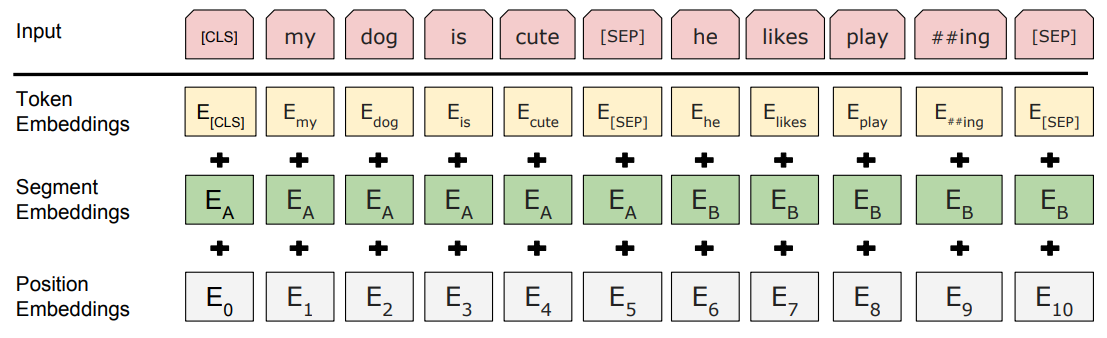
\includegraphics[scale=0.6]{img/bert/bert_input.png}
    \caption{Входные данные}
\end{figure}

Входные данные для обучения: пары предложений со  разделенных специальным токеном-разделителем [SEP] (рис 2.15). Чтобы модель могла легко различать эти предложения, в дополнение к токеновым и позиционным вложениям она использует вложения сегментов. Также BERT имеет 2 цели обучения, для которых используются некоторые специальные токены([MASK], [CLS]). \\

\begin{center}
    \textbf{Первая цель обучения обучения: Masked Language Modeling (MLM)}
\end{center}
Наиболее важной из двух целей обучения является цель моделирования замаскированного языка (MLM). На этапе обучения для MLM происходит следующее:
\begin{itemize}
    \item Выбирается несколько токенов (каждый токен выбирается с вероятностью 15\%)
    \item Выбранные токены заменяются на [MASK] с вероятности 80\%, случайный токен - 15\% и остается без изменений - 10\%
    \item Модель должна предсказать исходный токен
\end{itemize}

На рисунке ниже показан пример шага обучения для одного предложения.

\begin{figure}[h]
    \centering
    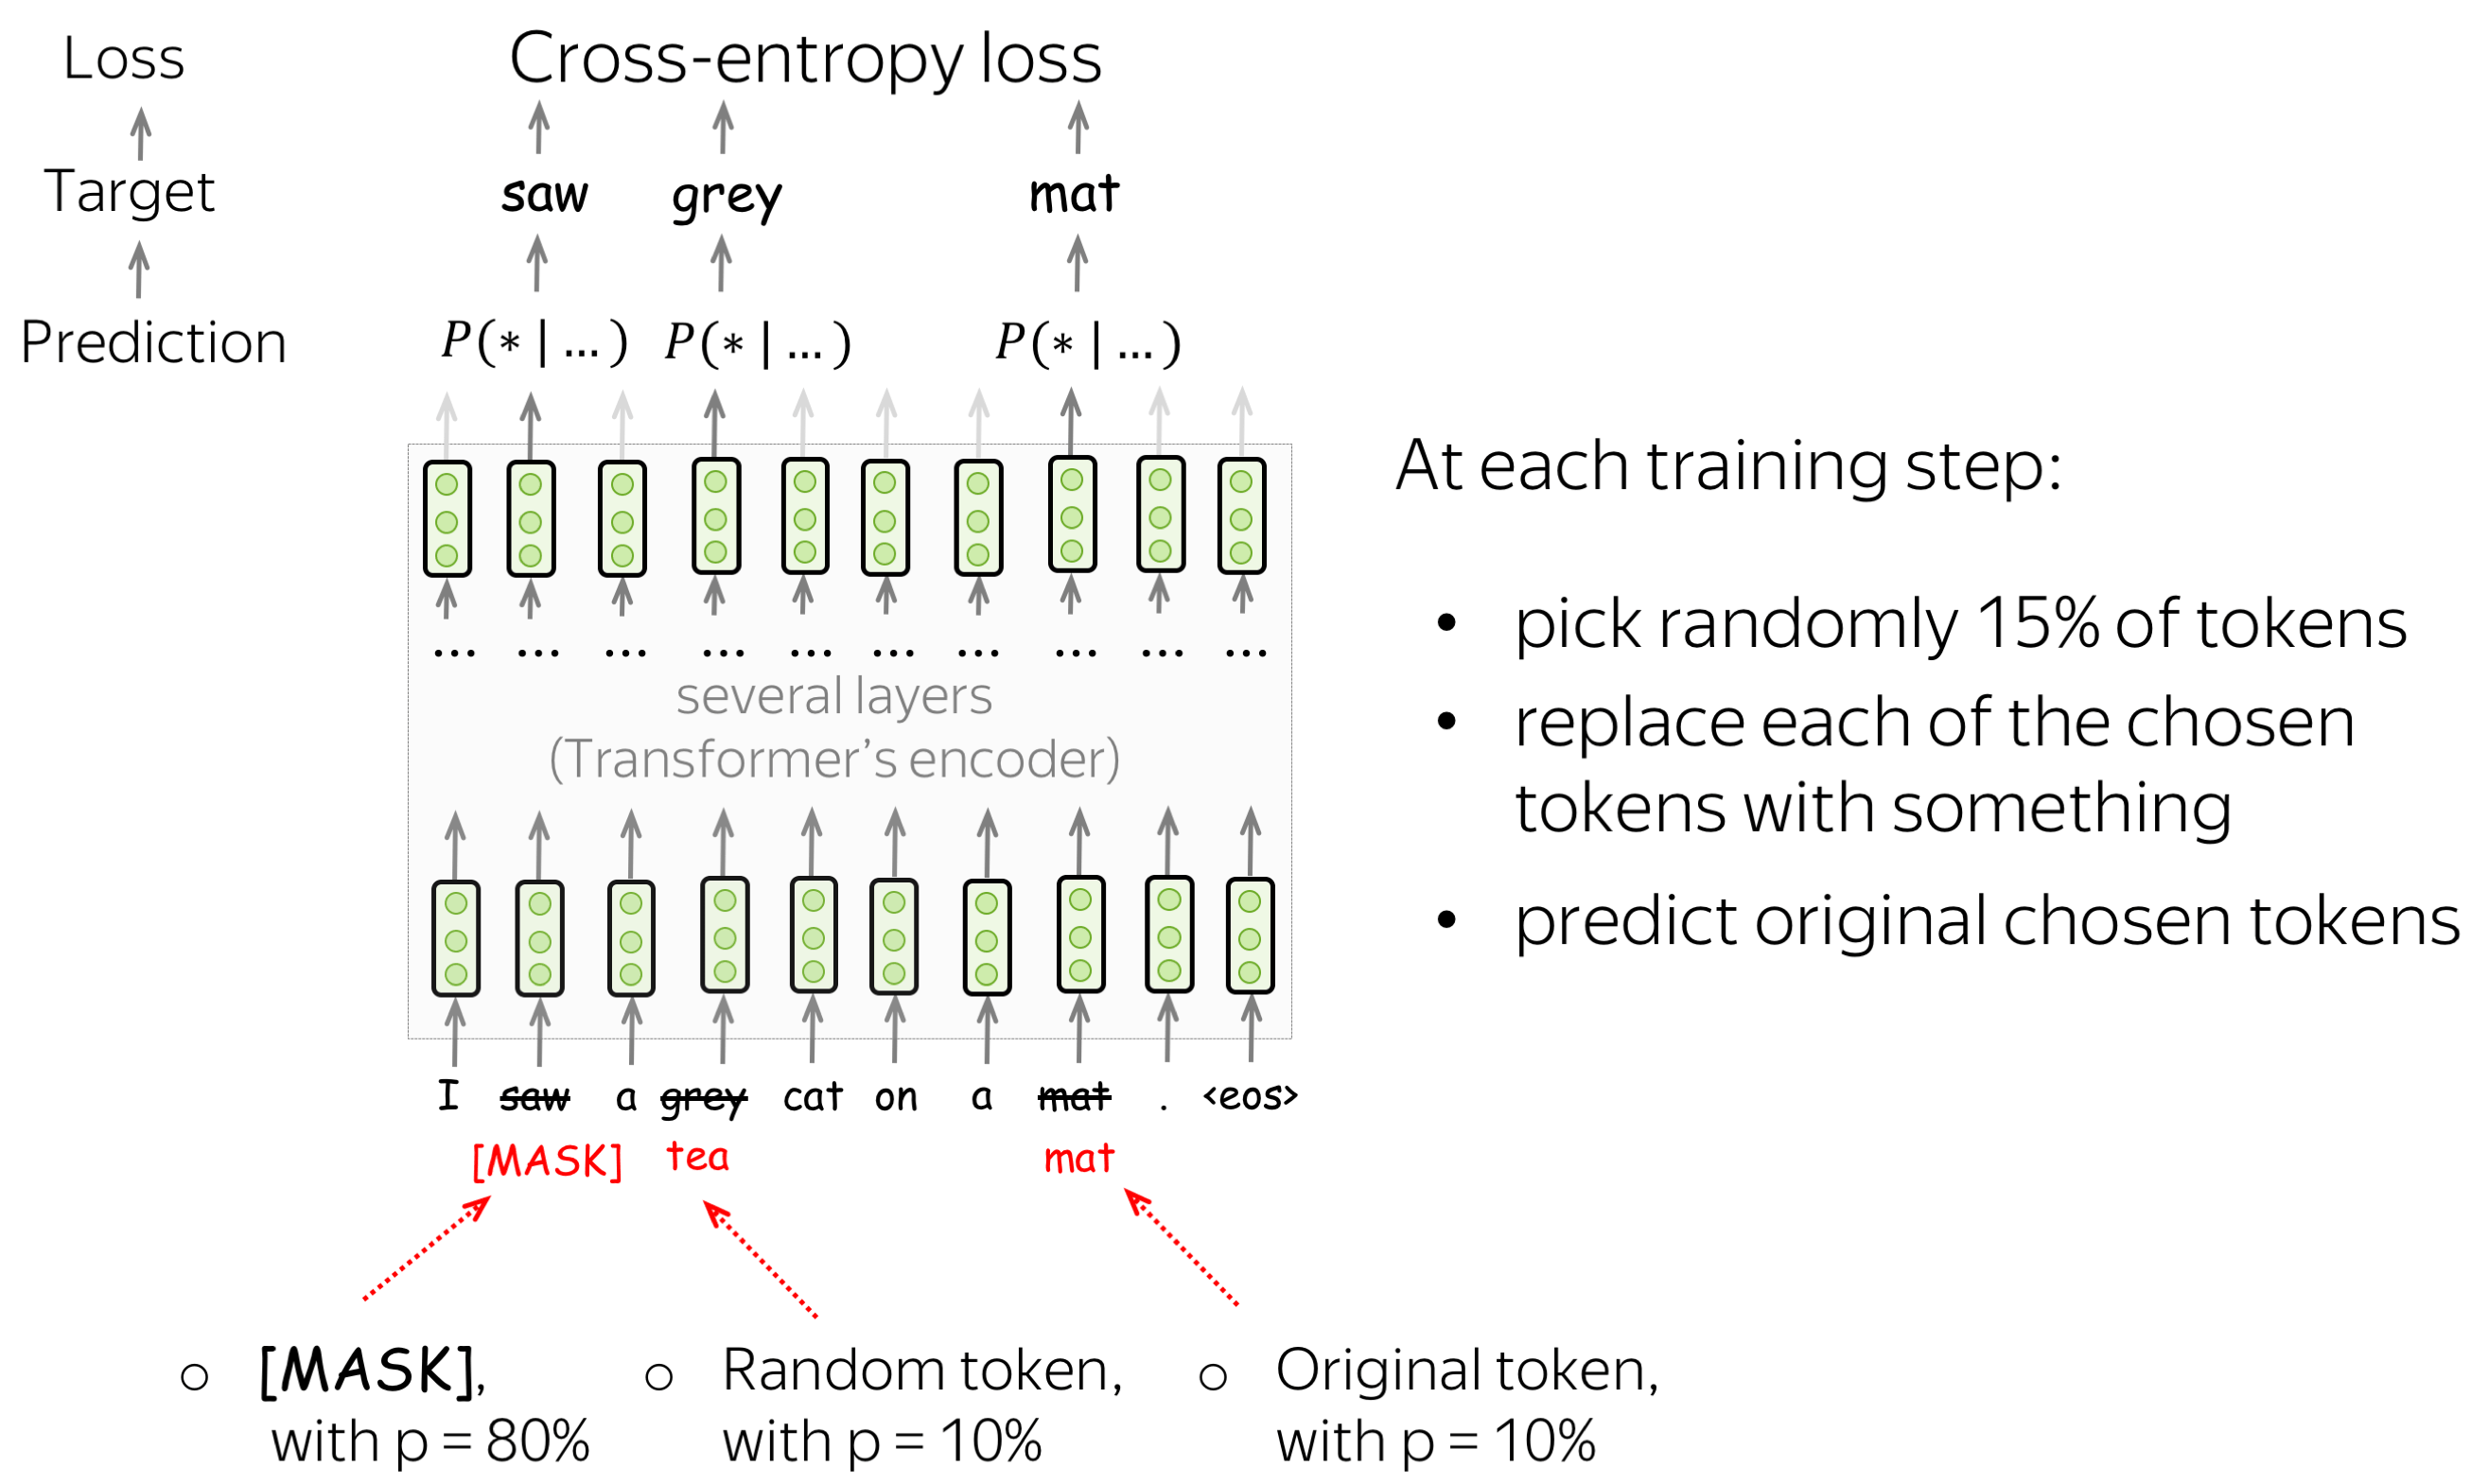
\includegraphics[scale=0.18]{img/bert/bert_tasks.png}
    \caption{Masked Language Modeling (MLM)}
\end{figure}
\newpage
\begin{center}
    \textbf{Вторая цель обучения обучения: Next Sentence Prediction (NSP)}
\end{center}

Задача «Предсказание следующего предложения» (NSP) представляет собой задачу бинарной классификации. На последнем уровне модели, исходя из токена [CLS], модель предсказывает, являются ли два предложения последовательными предложениями в некотором тексте или нет. В датасете для обучения, представленном в оригинальной статье сказанно, что при обучении 50\% примеров содержат последовательные предложения, извлеченные из обучающих текстов, а еще 50\% — случайную пару предложений.

Это задание учит модель понимать отношения между предложениями и позволяет BERT решать более сложные задачи.

\begin{center}
    Пример из исходного датасета:
\end{center}

Ввод: [CLS] мужчина пошел в [MASK] магазин [SEP] он купил галлон [MASK] молока [SEP]

Метка: Последовательные \\

Ввод: [CLS] мужчина пошел в магазин [MASK] [SEP] пингвин [MASK] летают \#\#less birds [SEP]

Метка: Непоследовательные\\

Следует также упомянуть, что BERT подходит для решения разных задач, ниже приведены основные типы задач:

\begin{itemize}
    \item Классификация отдельных предложений
          Для классификации отдельного предложения, вводятся токены предложения и [CLS] с классом предложения.
    \item Классификация пар предложений
          Для классифицикации пары предложений, вводятся токены предложений, как в обучении, и и [CLS] с классом предложения.
    \item Ответ на вопрос (Question answering)
          В задачах вопросов на ответы, на вход дают тект и вопрос. Ответ на этот вопрос содержится в исходном тексте, и задача состоит в том, чтобы найти отрывок из текста с ответом.
    \item Тэгирование слов в предложении
          В задачах тегирования прогнозируются теги для каждого токена. Например, в распознавании именованных объектов (NER) вы должны предсказать, является ли слово именованным объектом и его типом (например, местоположение, человек и т. д.).
\end{itemize}


\subsection{RoBERTa - улучшенная версия BERT}

Модель RoBERTa была предложена в книге RoBERTa: A Robustly Optimized BERT Pretraining Approach\cite{roberta:2019}. Он основан на модели Google BERT, выпущенной в 2018 году. Она основан на BERT и изменяет ключевые гиперпараметры, удаляя цель предварительного обучения в следующем предложении и обучая с гораздо большими мини-батчами и learning rate. \\

Список основных изменений представлен ниже:
\begin{itemize}
    \item Обучение большем объем данных (в 10 раз больше) и дольше по времени.
    \item Входные данные представляют собой более длинные последовательности, при оставшемся ограничении в 512 токенов, как и у BERT
    \item Динамическое маскирование токенов: токены маскируются по-разному в каждую эпоху, тогда как BERT делает это раз и навсегда
    \item Использование большого батча (относительно исходного BERT с батчем 256) при обучении модели
    \item Использование Byte-Pair Encoding с байтами в качестве субъединицы, а не с символами (из-за символов юникода)
\end{itemize}


\newpage
\section{Модель Wave2vec 2.0}

Фреймворк wave2vec 2.0\cite{w2v:2020} разработан для self-supervised обучения эмбеддингов на основе необработанных аудиоданных. Модель кодирует речевой звук с помощью многослойной сверточной нейронной сети, а затем маскирует участки результирующих скрытых речевых представлений, аналогично моделированию замаскированного языка (MLM), который был разобран в разделе про BERT. Скрытые представления передаются в Трансформер для построения контекстуализированных эмбеддингов, и модель обучается с помощью contrastive learning.


Как показано на рисунке ниже, модель обучается в два этапа. Первый этап проходит в режиме самоконтроля, который выполняется с использованием немаркированных данных и направлен на достижение наилучшего возможного представления речи. Вы можете думать об этом так же, как вы думаете о встраивании слов. Эмбеддинги слов также направлено на достижение наилучшего представления естественного языка. Основное отличие заключается в том, что Wav2Vec 2.0 обрабатывает аудио вместо текста.

Вторая фаза обучения - это контролируемая тонкая настройка, в ходе которой помеченные данные используются для обучения модели предсказывать определенные слова или фонемы (наименьшая возможная звуковая единица в определенном языке).

\begin{figure}[h]
    \centering
    \includegraphics[scale=0.8]{img/wave2vec/w2v_stages.png}
    \caption{Этабы обучения wave2vec}
\end{figure}

Архитектура окончательной модели, используемой для прогнозирования, состоит из трех основных частей:

\begin{itemize}
    \item Cверточные слои, которые обрабатывают входные данные необработанной формы сигнала для получения скрытого представления - Z,
    \item Трансформер из n слоев, создающий эмбеддинги с контекстом - C,
    \item линейная проекция на выходные данные - Y
\end{itemize}

\subsection{Контрастивное обучение}
Контрастивное обучение - это концепция, в рамках которой входные данные преобразуются двумя различными способами. После этого модель обучается распознавать, являются ли два преобразования входных данных по-прежнему одним и тем же объектом. В Wav2Vec 2.0 трансформаторные слои являются первым способом преобразования, второй осуществляется путем квантования, что будет объяснено в дальнейшей части этой статьи. Более формально, для замаскированного скрытого представления $z_{t}$ мы хотели бы получить такое контекстное представление $c_{t}$, чтобы иметь возможность угадать правильное квантованное представление $q_{t}$ среди других квантованных представлений.

\begin{figure}[h]
    \centering
    \includegraphics[scale=0.25]{img/wave2vec/wave2vec.png}
    \caption{Входные данные}
\end{figure}

\subsection{Квантизация}
Квантизация - это процесс преобразования значений из непрерывного пространства в конечный набор значений в дискретном пространстве.

У нас есть вектор представления скрытой речи $z_{t}$ охватывает несколько фонем. Число фонем в языке конечно. Более того, число всех возможных пар фонем конечно. Это означает, что они могут быть идеально представлены одним и тем же скрытым речевым представлением. Кроме того, их число конечно, поэтому мы можем создать "кодовую книгу", содержащий все возможные пары фонем. Затем квантование сводится к выбору правильного кодового слова из "кодовую книгу". Однако вы можете себе представить, что количество всевозможных звуков огромно. Чтобы упростить обучение и использование, авторы Wav2Vec 2.0 создали G кодовых книг, каждая из которых состоит из V кодовых слов. Чтобы создать квантизированное представление, следует выбрать лучшее слово из каждой кодовой книги. Затем выбранные векторы объединяются и обрабатываются линейным преобразованием для получения квантизированное представления.

\begin{figure}[h]
    \centering
    \includegraphics[scale=0.7]{img/wave2vec/w2v_books.png}
    \caption{Выбор токена их кодовых книг}
\end{figure}


Выбор правильного кодовго представления выбирается с помощью Gumbel softmax:

\begin{center}
    $p_{g, v} = \frac{exp{\frac{sim(l_{g, v} + n_{v})}{\tau}}}{\displaystyle\sum_{k=1}^{V} exp{\frac{l_{g, k} + n_{k}}{\tau}}}$,
    где
    \begin{itemize}
        \item sim — косинусное сходство,
        \item l — логиты, полученные свертками,
        \item $n_{k} = -log(-log(gl))$,
        \item $u_{k}$ - выборки из равномерного распределения U(0, 1),
        \item $\tau$ - температура
    \end{itemize}
\end{center}

Поскольку это задача классификации, функция softmax представляется естественным выбором для выбора наилучшего кодового слова в каждой кодовой книге. Gumbel softmax поставляется с двумя улучшениями: рандомизацией и температурой $\tau$. Благодаря рандомизации модель более охотно выбирает разные кодовые слова во время обучения, а затем обновляет их веса. Важно, особенно в начале обучения, не допускать использования только подмножества кодовых книг.

\subsection{Diversity loss (Потеря разнообразия)}

Потеря разнообразия - это своего рода метод регуляризации. Авторы установили G=2 кодовых книги с V=320 кодовыми словами в каждой кодовой книге. Теоретически это дает $320 \cdot 320 = 102400$ возможных квантованных представлений. Но в процессе обучения можно  столкнутся с проблемой того, что модель использовать все эти возможности. Она научится использовать, например, только 100 кодовых слов из каждой кодовой книги и растратит весь потенциал кодовой книги впустую. Вот почему потеря разнообразия может быть полезной. Он основан на энтропии, которая может быть вычислена по следующей формуле:

\begin{center}
    $H(x) = - \displaystyle\sum_{x} P(x)\cdot log(P(x))$, где
\end{center}

$x$ — возможный результат действия дискретной случайной величины $X$,

$P(x)$ — вероятность события $x$. \\

Энтропия принимает максимальное значение, когда распределение данных является равномерным. В случае wave2vec это означает, что все кодовые слова используются с одинаковой частотой. С помощью этого производится вычисление энтропию каждой кодовой книги по всей серии обучающих примеров, чтобы проверить, используются ли кодовые слова с одинаковой частотой. Максимизация этой энтропии побудит модель использовать преимущества всех кодовых слов. Максимизация равна минимизации отрицательной энтропии, которая является потерей разнообразия.\\

\begin{center}
    $L_{d} = \frac{1}{GV} \cdot (-H(\overline{p}_{g})) = \frac{1}{GV}\displaystyle\sum_{g=1}^{G}\displaystyle\sum_{v=1}^{V} \overline{p}_{g, v} \cdot log(\overline{p}_{g, v})$
\end{center}


\newpage
\chapter{Практическая часть}

Основной задачей в работе будет классификация видео на наличие юмора с использованием разных моделей для разных модальностей.
Для работы с разными модальностями будут использованы 3 модели, которые были описаны в теоретической части:
\begin{itemize}
    \item Wave2Vec - извлечение аудио признаков,
    \item BERT - извлечение текстовых признаков,
    \item TimeSFormer - извлечение признаков из видео фрагментов,
\end{itemize}

Сначала модели попробуют предсказать классы в своих модальностях, после чего их предсказания будут обработаны вместе для улучшения результатов.

\section{Классификация по одной модальности}

Для извлечения признаков, как уже было описано, будут использоваться 3 различные модели. В силу ограниченных вычислительных мощностей, будут взяты предобученные модели с \href{https://huggingface.co/}{Hugging Face} и дообучены на наших данных.

Так как у нас ровное кол-во наблюдений положительного и отрицательного классов, делим выборку 70\% на дообучение и 30\% валидацию с одинаковым кол-вом примеров разных классов в обеих подвыборках.

Для каждой модели начала посчитаем качество модели по 3 метрикам: Accuracy (из-за отличной балансировки, можем использовать обычную accuracy), Precision, Recall.

\begin{itemize}
    \item Для работы с текстом будем использовать RoBERTa из библиотеки моделей HuggingFace: \href{https://huggingface.co/roberta-base}{roberta-base}.
    \item Для работы с аудио будем использовать Wave2vec2 из библиотеки моделей HuggingFace: \href{https://huggingface.co/facebook/wav2vec2-base}{wav2vec2-base}.
    \item Для работы с видео будем использовать Wave2vec2 из библиотеки моделей HuggingFace: \href{https://huggingface.co/facebook/timesformer-base-finetuned-k400}{timesformer-base}.
\end{itemize}

С помощью предлагаемых Hugging Face интрументов, сделаем дообучение моделей под нашу задачу. \\

\subsection{Результаты}

\textbf{Далее в таблицах с результатами модальности будут называться в сокращенном виде: Текст - Т, Аудио - А, Видео - В.} \\

Результаты классификации по одной модальности: \\

\begin{center}
    \begin{tabular}{ |c||c|c|c|}
        \hline
        \multicolumn{4}{|c|}{Классификация по тексту} \\
        \hline
        Модальность & Accuracy & Precision & Recall   \\
        \hline
        Т           & 0.71377  & 0.70563   & 0.75064  \\
        В           & 0.47836  & 0.50600   & 0.59729  \\
        А           & 0.50885  & 0.57865   & 0.78420  \\
        \hline
    \end{tabular} \\
\end{center}



TimeSFormer показывает достаточно низкие значени метрик, относительно других моделей. Такие результаты связаны со спецификой задачи, моедль не фоксируется только на человеке, но на всем видеофрагменте. Возможным решением станет использование других моделей или инструментов, которые будут обрабатывать именно человека на видео.

Wave2vec показывает хороший recall (т.е модель хорошо угадывает, класс с юмором), но accuracy все еще плохой.

По результатам можем сделать вывод, что самым подходящей для детекции юмора оказалась текстовая модальност, с которой работала RoBERTa. Действительно по тексту легче всего понять, есть ли шутка, потому что не надо обрабатывать много второстепенной информации, как в видео, и "поведение"\ голоса разных людей во время шутки, как на аудио.

\section{Классификация видео с использованием нескольких модальностей}

Теперь попробуем собирать вместе голосование моделей в разных модальностях, сначала будем брать все комбинации 2 модальностей, а потом возьмем 3 модальности.

Подсчет результатов будем производить двумя разными сопобами:
\begin{itemize}
    \item Посчитать среднюю вероятность
    \item Выбирать голосованием, каждой модели за класс
\end{itemize} \\

\subsection{Результаты}

Результаты экспериментов с подсчетом средней вероятности: \\

\begin{center}
    \begin{tabular}{ |c||c|c|c| }
        \hline
        Модальности & Accuracy & Precision & Recall  \\
        \hline
        А + В       & 0.49737  & 0.50512   & 0.60373 \\
        А + Т       & 0.71377  & 0.70488   & 0.75257 \\
        В + Т       & 0.63573  & 0.63569   & 0.66559 \\
        А + В + Т   & 0.63081  & 0.62862   & 0.67074 \\
        \hline
    \end{tabular}
\end{center} \\

В голосованиях в парах и тройке результаты лучше, чем у А и В по одиночке.
А + Т слегка улучшает результат RoBERTa в одиночку, а в остальных парах и тройке, результаты улучшаются, но не достигают RoBERTa.


При спорных ситуациях в голосованием по классам, решающий голос за модальностями с лучшим результатом в прошлой частью (т.е. TimeSFormer имеет самый слабый голос, затем Wave2Vec и самый сильный голос у RoBERTa).

Результаты экспериментов с голосованием по классам: \\

\begin{center}
    \begin{tabular}{ |c||c|c|c|}
        \hline
        Модальности & Accuracy & Precision & Recall  \\
        \hline
        А + В       & 0.49737  & 0.50512   & 0.60373 \\
        А + Т       & 0.71377  & 0.70563   & 0.75064 \\
        В + Т       & 0.71377  & 0.70563   & 0.75064 \\
        А + В + Т   & 0.50885  & 0.50885   & 1.0     \\
        \hline
    \end{tabular}
\end{center} \\

Здесь можно заметить, т.к. текст имеет решщающий голос, то в парах с текстом результаты одинаковые.
В А + В + Т интересно заметить, что recall равен 1.0. Тоесть наша "тройка"\ относит все сэйплы к одному классу.


\chapter{Заключение}

В ходе проделанной работы были прочитаны статьи в разделе нейронных сетей, изучен механизм внимания и архитектура Трансформер с теоретической точки зрения. Также изучены модели, в основе которых лежит Трансформер: RoBerta, используемая для работы с текстовой модальностью, Wave2vec2, используемая для работы с звуковой модальностью, и TimeSFromer, используемая для работы с визуальной модальностью.

Далее были проведены эксперименты  на датасете UrFunnny с каждой из моделей. Изучив результаты можно увидеть, что RoBERTa показыает самые хорошие результаты. Предположения, почему получились такие результаты было сделано в пунке 3.1.1 под таблицей с результатами.

Что касается совмещения результатов моделей (голосование по вероятностям и финальным лэйблам), аудио и текст вместе улучшают результат RoBERTa в одиночку.

Для работы с моделями, обучение и инференс, был изучен фрэймворк HuggingFace, имеющий большую популярность в сфере глубокого обучения. Кроме того были использованы язык программирования Python, PyTorch - бекэнд для нейронных сетей, а также вспомогательные библиотеки librosa (работа со звуком) и Numpy.

Следующим шагом в исследовании детекции юмора может стать объединением моделей в одну, на примере CLIP от openAI или улучшение моделей в аудио и видео модальностях.




\putbibliography %Вместо этой команды будет вставлена библиография

\end{document}